\section{Simulations}

\subsection{Implementation notes}

\subsection{Transfer orbit}

\subsection{Around Lagrange L2}

We now consider the reduced 3-body problem, like in \ref{sec:3body_reduced}. The simulations are done in the \(\mathcal R'\) reference frame, placing Webb at the Lagrange L2 point given in \ref{sec:lagrange_L2} and giving the satelite an initial downwards speed \(\dot y' = -0.1\) m/s. We will first analyse the convergence of both methods.

Due to the nature of the adaptative timestep method, the convergence order against \(\frac{1}{n_\textrm{steps}}\) will be analysed. The results wit the initial conditions given above are reported in \autoref{fig:lagrange_conv}. Both methods converge with order 5 

\begin{figure}[h]
    \centering
    \begin{subfigure}{0.45\linewidth}
        \centering
        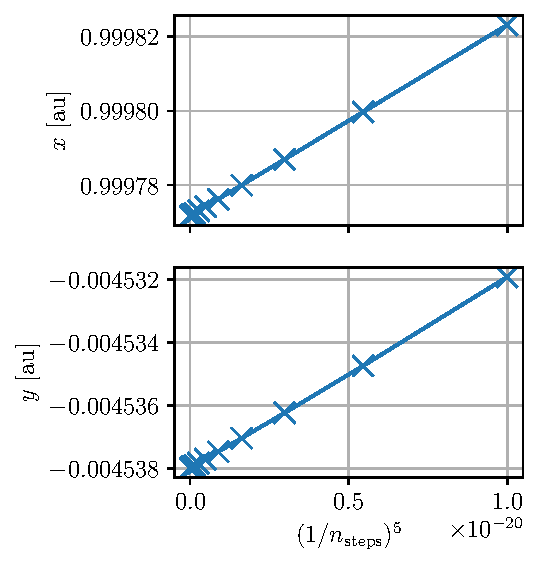
\includegraphics[width=\linewidth]{figures/lagrange_convergence_fixed.pdf}
        \caption{Fixed \(\dd t\) method}
        \label{fig:lagrange_conv_fixed}
    \end{subfigure}
    \begin{subfigure}{0.49\linewidth}
        \centering
        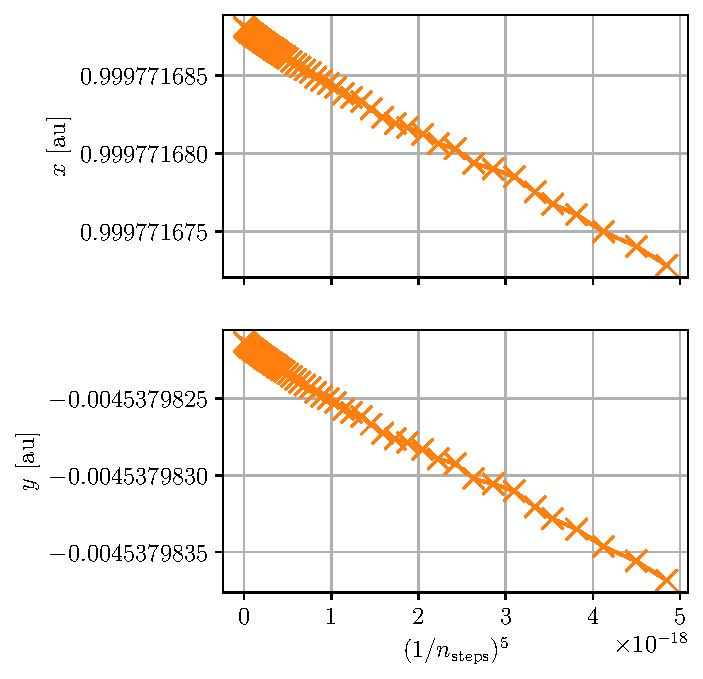
\includegraphics[width=\linewidth]{figures/lagrange_convergence_adapt.pdf}
        \caption{Adaptative \(\dd t\) method}
        \label{fig:lagrange_conv_adapt}
    \end{subfigure}
    \caption{Final position convergence starting from L2 with initial downwards speed \(\dot y' = -0.1\) m/s for both methods. \(n_\textrm{steps}\) was varied from \(10^4\) to \(10^6\) for the fixed timestep method and the tolerance \(\varepsilon\) was varied from \(10^{-5}\) to \(10^{-1}\) for the adaptative method.}
    \label{fig:lagrange_conv}
\end{figure}
